%\documentclass[11pt,a4paper]{report}


% The Beamer class comes with a number of default slide themes
% which change the colors and layouts of slides. Below this is a list
% of all the themes, uncomment each in turn to see what they look like.

%\usetheme{default}
%\usetheme{AnnArbor}
%\usetheme{Antibes}
%\usetheme{Bergen}
%\usetheme{Berkeley}
%\usetheme{Berlin}
%\usetheme{Boadilla}
%\usetheme{CambridgeUS}
%\usetheme{Copenhagen}
%\usetheme{Darmstadt}
%\usetheme{Dresden}
%\usetheme{Frankfurt}
%\usetheme{Goettingen}
%\usetheme{Hannover}
%\usetheme{Ilmenau}
%\usetheme{JuanLesPins}
%\usetheme{Luebeck}
%\usetheme{Madrid}
%\usetheme{Malmoe}
%\usetheme{Marburg}
%\usetheme{Montpellier}
%\usetheme{PaloAlto}
%\usetheme{Pittsburgh}
%\usetheme{Rochester}
%\usetheme{Singapore}
%\usetheme{Szeged}
%\usetheme{Warsaw}

\documentclass[10pt,spanish]{beamer}
\usepackage{float}
\usepackage[export]{adjustbox}
\usepackage[nodisplayskipstretch]{setspace}
\usepackage{pdfpages}
\usepackage{tikz}    
\usetheme{metropolis}
\usepackage{appendixnumberbeamer}
\usepackage[normalem]{ulem}
\usepackage{eurosym}
\usepackage{booktabs}
\usepackage[scale=2]{ccicons}
\usepackage[utf8]{inputenc}
\usepackage{soul}
\usepackage{mathabx}
\usepackage{graphicx}
\usepackage{pgfplots}
\usepgfplotslibrary{dateplot}
 \usepackage{relsize}
\usepackage{xspace}
\usepackage{caption}
\usepackage{amsmath} % for \boxed{}
\usepackage{graphicx}
\usepackage{graphicx}
\usepackage{accents}
\newlength{\dhatheight}
\usepackage{hyperref}
\hypersetup{
    colorlinks=true,
    linkcolor=blue,
    filecolor=magenta,      
    urlcolor=blue,
}
 \setbeamertemplate{itemize items}[ball]
\urlstyle{same}
\newcommand{\themename}{\textbf{\textsc{metropolis}}\xspace}
\usepackage{tikz-cd}
\usetikzlibrary{matrix}

\usepackage{amsmath}
\usepackage{amsfonts}
\usepackage{listings}
\usepackage{graphicx} % Required for including images
\usepackage[font=small,labelfont=bf]{caption} % Required for specifying captions to tables and figures
\usepackage{hyperref}
\usepackage[utf8]{inputenc}
\usepackage[spanish]{babel}
\usepackage{amsthm}
\usepackage{graphicx}
\usepackage{amssymb}
\usepackage{amssymb}
\usetikzlibrary{arrows,positioning}

\usepackage{enumitem}   
\usepackage{xspace}


% As well as themes, the Beamer class has a number of color themes
% for any slide theme. Uncomment each of these in turn to see how it
% changes the colors of your current slide theme.

%\usecolortheme{albatross}
%\usecolortheme{beaver}
%\usecolortheme{beetle}
%\usecolortheme{crane}
%\usecolortheme{dolphin}
%\usecolortheme{dove}
%\usecolortheme{fly}
%\usecolortheme{lily}
%\usecolortheme{orchid}
%\usecolortheme{rose}
%\usecolortheme{seagull}
%\usecolortheme{seahorse}
%\usecolortheme{whale}
%\usecolortheme{wolverine}

%\setbeamertemplate{footline} % To remove the footer line in all slides uncomment this line
%\setbeamertemplate{footline}[page number] % To replace the footer line in all slides with a simple slide count uncomment this line

%\setbeamertemplate{navigation symbols}{} % To remove the navigation symbols from the bottom of all slides uncomment this line


\usepackage[utf8]{inputenc}
\usepackage{graphicx}

\usepackage{amsmath,amsthm,amssymb,latexsym,amsfonts}


\setlength{\parindent}{15pt}
\usepackage{subfig}
\usepackage{hyperref}
\usepackage{graphicx} % Allows including images
\usepackage{booktabs} % Allows the use of \toprule, \midrule and \bottomrule in tables

\usepackage{bm}
\newcommand{\doublehat}[1]{%
    \settoheight{\dhatheight}{\ensuremath{\hat{#1}}}%
    \addtolength{\dhatheight}{-0.35ex}%
    \hat{\vphantom{\rule{1pt}{\dhatheight}}%
    \smash{\hat{#1}}}}
%\title{Probar que un predicado es primitivo recursivo sin marearse}
%\author{Guillermo Mosse}
\def\m{^{-1}}
\def\key#1{\{#1\}}

\def\N{\mathbb{N}}
\def\F{\mathbb{F}}

\def\b{$\mathlarger{\mathlarger{\mathlarger{\mathlarger{\mathlarger{\cdot}}}}}$}

\begin{document}

%$\omega^{\omega^\omega} \approx \overline{F_2}$
\title{Final Álgebra III: Hacia la clausura algebraica de $\F_2$}
\subtitle{\tiny{¡Los ordinales son útiles!}}
% \date{\today}
\date{}
\author{Guillermo Mosse}

\maketitle



% En esta charla pretendo dar un esbozo de cómo es la construcción (explícita) de la clausura algebraica de $\mathbb{F}_2$ vía los ordinales.

% Para meternos en el tema, primero voy a dar una introducción corta sobre ordinales, con algunos resultados fundamentales.

% Los ordinales son identificaciones de los buenos órdenes.

% Así como los cardinales son representantes de la relación de equivalencia entre conjuntos dados porque exista una biyección entre ellos,
% los ordinales son representantes de la relación de equivalencia de los conjuntos bien ordenados dada porque exista un isomorfismo de orden.

% Ahora bien, eso suena bastante abstracto, esotérico, poco manejable.

% La construcción clásica de los ordinales es la de Von Neumann:



\begin{frame}{¿Qué son los ordinales?}

% La construcción es inductiva
% Empezamos por el ordinal 0, que codifica al conjunto vacío
% El 1 va a ser el conjunto de los ordinales anteriores, que es solamente el 0
% El 2 va a ser el conjunto de los ordinales anteriores, o sea, el 0 y el 1
% Y así seguimos

$$ 0 = \emptyset $$ \pause
$$ 1 = \key{0}$$ \pause
$$ 2 = \key{0,1}\ \ = 1 \cup \key{1} $$\pause
$$ 3 = \key{0,1,2} = 2 \cup \key{2}$$\\
$$ 4 = \key{0,1,2,3} = 3 \cup \key{3}$$

$$...$$

\end{frame}



\begin{frame}{Más ordinales}

% Dado un conjunto de ordinales yo puedo tomar la unión de todos para definir un nuevo ordinal. Así es como me salgo de $\N$. Por ejemplo, defino $\omega$ (que es $\N$, en el fondo) como la unión de todos los ordinales que son números naturales. Y así uno puede seguir infinitamente, obteniendo $\omega+1, \omega+2,..., \omega \cdot 2, \omega \cdot 3,...$ pero la construcción nunca termina, porque siempre que tenemos un proceso infinito de construcción de ordinales podemos considerar la unión de todos para obtener un nuevo ordinal.


$$5 = \key{0,1,2,3,4} = 4 \cup \key{4}$$\\
$$6 = \key{0,1,2,3,4,5} = 5 \cup \key{5}$$ \pause
$$\omega = \key{0,1,2,3,...} \leftarrow\text{ es un ordinal límite}$$ \pause
$$\omega + 1 = \key{0,1,...,\omega} = \omega \cup \key{\omega}$$ \\
$$\omega + 2 = \key{0,1,...,\omega, \omega+1} = \omega +1 \cup \key{\omega+1}$$\\
$$...$$ \pause
$$\omega + \omega = \omega \cdot 2 = \key{0,1,...,\omega, \omega+1, \omega+2,...}$$


% Los ordinales son realmente inconmensurables, y uno al construir ordinales cada vez más grandes por medio de métodos cada vez más esotéricos, va perdiendo la noción de qué buen orden representa el orden que consigue. De paso, de eso se trata mi tesis: de darle más sustancia a algunos especiales especiales e intentar bajar las cosas un poco más a tierra.

\end{frame}

\begin{frame}{Operaciones}
	Suma y Producto de \textbf{ordinales} $\approx$ Suma y producto de \textbf{cardinales} \pause


% Mhm, e insisto, a los ordinales me parece que no hay que pensarlos como clases de equivalencia de los buenos órdenes salvo que no haya alternativa (por ejemplo, para alguna demo). Hay que pensarlos como una extensión de la aritmética en $\mathbb{N}$. Y, en ese sentido, uno puede operar con ordinales. Existen la suma y producto de ordinales, que generalizan las de $\N$, y son super parecidas a la de cardinales

% La suma de ordinales es la unión de los conjuntos que representan

% El producto es el orden que resulta de mirar el orden lexicográfico del producto de ordinales.
	
	
	¡La exponenciación es distinta!

% La exponenciación es distinta a la de cardinales.


% En cardinales, ${\aleph_0}^{\aleph_0}$ te devuelve un ordinal no numerable y en ordinales no

% No vamos a usar mucho la exponenciación, pero si ves alguna exponenciación es un ordinal numerable

% Si la exponenciación de cardinales era que $\alpha^\beta$ eran las funciones de $\beta$ en $\alpha$ la de ordinales era ver las funciones de soporte finito. Esto se hace para que el conjunto obtenido tenga un buen orden (si considerás todas las funciones no funciona eso)

% En general las operaciones que existen para ordinales te devuelven todos ordinales numerables
	
	\begin{itemize}
		\item[$\bullet$]$\alpha^0:= 1$
		\item[$\bullet$]$\alpha^{\beta + 1} := \alpha^\beta \cdot \alpha$
		\item[$\bullet$]Si $\beta$ es límite, $\alpha^\beta = \underset{\lambda < \beta}{\cup} \alpha^\lambda$.
	\end{itemize}
	
\end{frame}

% Bueno, estas son algunas representaciones gráficas de ordinales. Se llaman "Matchsticks", porque son palitos, básicamente

\begin{frame}{Matchsticks: $\omega$}
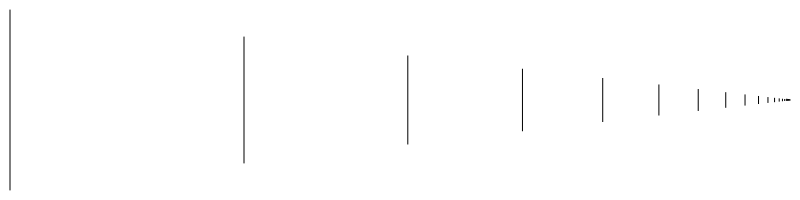
\includegraphics[scale=0.4]{w.png}
\end{frame}

\begin{frame}{$\omega^2$}
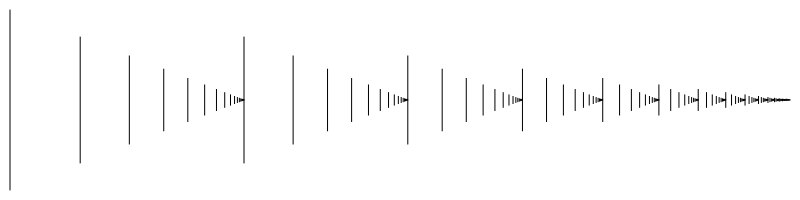
\includegraphics[scale=0.4]{w^2.png}
\end{frame}

\begin{frame}{$\omega^\omega$}
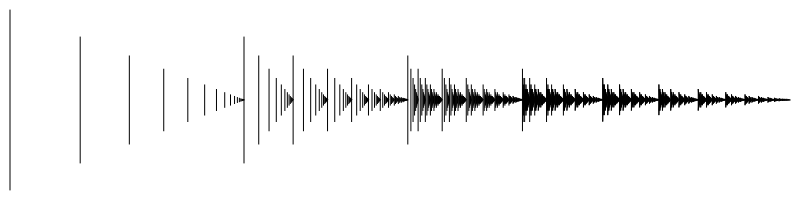
\includegraphics[scale=0.4]{w^w.png}
\end{frame}

\begin{frame}{Una representación gráfica hasta $\omega^\omega$}
	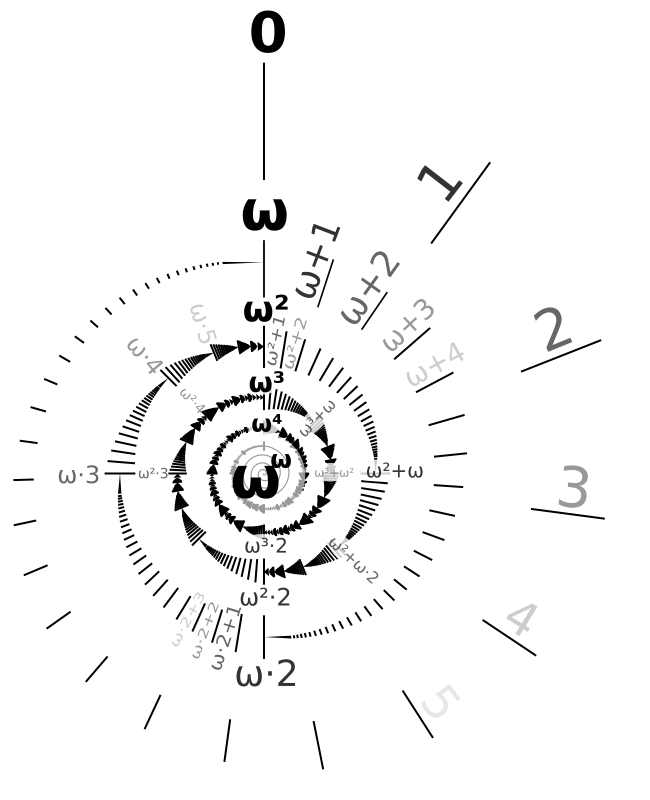
\includegraphics[scale=0.42]{spiral.png}
\end{frame}

\begin{frame}{$\omega^{\omega^\omega}$ (¡INENTENDIBLE!)}
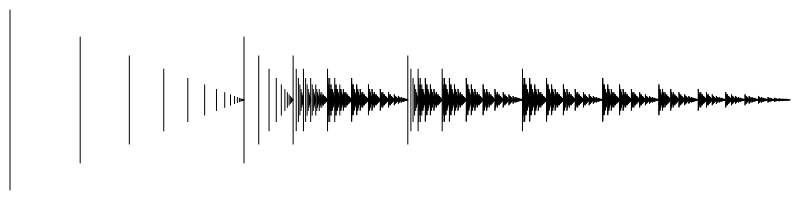
\includegraphics[scale=0.4]{w^w^w.png}
\end{frame}

\begin{frame}{Los ordinales como algo efectivo}

	% Yo cuando empecé a encarar el tema me sorprendí de poder decir las palabras "ordinales" y "método efectivo" en la misma oración.
	
	% Pero de a poco me fue cayendo la ficha: hay algo muy especial de los ordinales, que es que todo ordinal es un buen orden y, más aun, la clase de todos los ordinales también forma un buen orden.
	
\pause	Toda secuencia descendente de ordinales eventualmente termina.

	Equivalentemente, todo conjunto tiene un mínimo. Esto nos permite usar un esquema inductivo para probar propiedades sobre los ordinales.

\end{frame}

\begin{frame}{Forma normal de Cantor}

Todo ordinal $0 \neq \beta$ que nos va a interesar (o sea, no muy grande) admite una expresión de la siguiente forma:

$$\beta = \omega^{\alpha_1} \cdot m_1 + ... + \omega^{\alpha_k} \cdot m_k$$

con $\beta > \alpha_1 > ... > \alpha_k$, y $m_i \in \N$

Esto es una descomposición de $\beta$ en ordinales más chicos que él. \bigskip \pause

Además, uno puede hacer lo mismo con los $\alpha_i$... \pause

% Además, los $\alpha_i$ también se van a poder descomponer en ordinales más chicos. Esta cadena de descomposiciones me da una secuencia de ordinales decrecientes $\beta_1 > \beta_2 > ....$ Ahora, al principio vimos que cada ordinal es el conjunto de ordinales más chicos que él. $\forall\i > 1, \beta_i \in \beta_1$, que es un buen orden. Entonces eventualemente la secuencia termina, no puede descender infinitamente. Esto quiere decir que esta descomposición que hacemos termina.

% Notemos el parecido con $\N$, que también está bien ordenado y por eso podemos factorizar en primos.

% Lo que obtenemos es ordinales escritos como arbolitos, usando el símbolo $\omega$, y números naturales.

Algunos ejemplos:

$\omega\textbf{,}\ \ \omega^\omega \cdot 2\textbf{,}\ \ \omega^{\omega^2} + \omega^\omega + 4\textbf{,}\ \ \omega^{\omega^{\omega^2} + 2}$

% Al final del día, lo que importa de todo esto es que podemos operar y comparar ordinales de manera efectiva porque tenemos una notación para ellos. (No vamos a ver cómo se opera pero es muy fácil). En ese sentido los ordinales son una extensión de la aritmética en $\N$. Las operaciones pierden algunas propiedades (como conmutatividad) pero en general se puede operar etc.

\end{frame}

\begin{frame}{El producto no es conmutativo}
\pause
$2\cdot \omega$ es así:
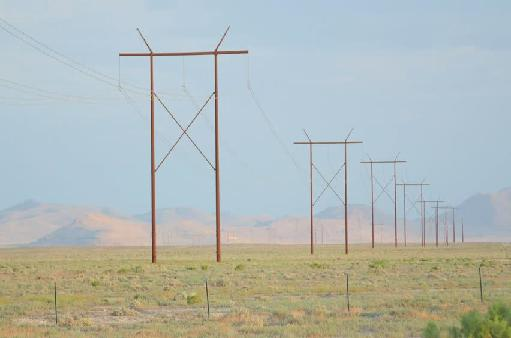
\includegraphics[scale=0.42]{2w_n.jpg}


, y $\omega$ es así:
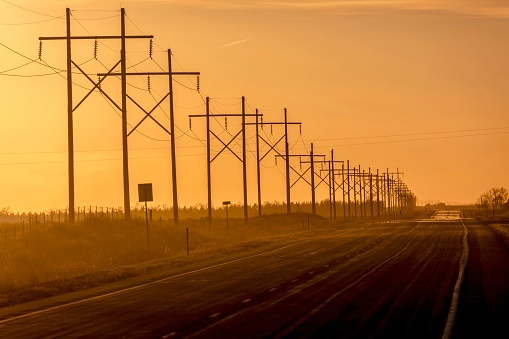
\includegraphics[scale=0.42]{w_n.png}

\end{frame}

\begin{frame}{El producto no es conmutativo (Cont)}
	Mientras que: $\omega \cdot 2$ es así:
	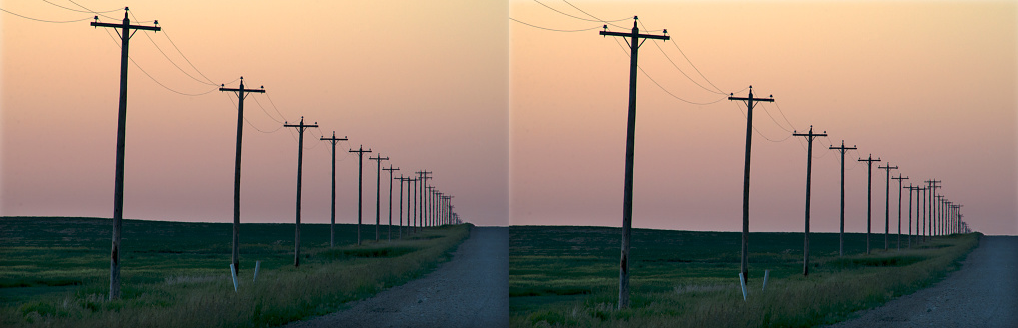
\includegraphics[scale=0.42]{w2.png}
\end{frame}

\begin{frame}{Las operaciones naturales de Conway}



$$\mathlarger{\mathlarger{\mathlarger{+ \rightarrow \oplus}}}$$


$$\mathlarger{\mathlarger{\mathlarger{\cdot \rightarrow \otimes}}}$$


% Las operaciones clásicas de ordinales, que podemos denotar [PIZARRÓN] + y .
% no son conmutativas. (ON,+,.) no forma un cuerpo, ni siquiera un grupo.

% Conway definió otra suma y otro producto, las llamadas "operaciones naturales" de ordinales. En realidad estas operaciones ya se usaban mucho en teoría de juegos y él las extendió a todo ON.

% Él buscaba las operaciones más simples que hicieran de ON un cuerpo.

% Restrinjámonos primero a los números naturales.
% Supongamos que estamos armando la tabla de doble entrada de la suma de ordinales.
% Y que supongamos que ya están definidos $\alpha'+\beta, \alpha + \beta'$ (explicar los primas) entonces $\alpha+\beta$ es el ordinal más chico consistente con la tabla de suma de algún cuerpo (que contenga a los elementos). Lo mismo va a pasar con la tabla de multiplicación.

%PIZARRÓN: hacer ejemplo en el pizarrón. Como 1+1=0, ya queda de entrada que el cuerpo va a ser de característica 2.

\end{frame}

\begin{frame}
\begin{figure}
	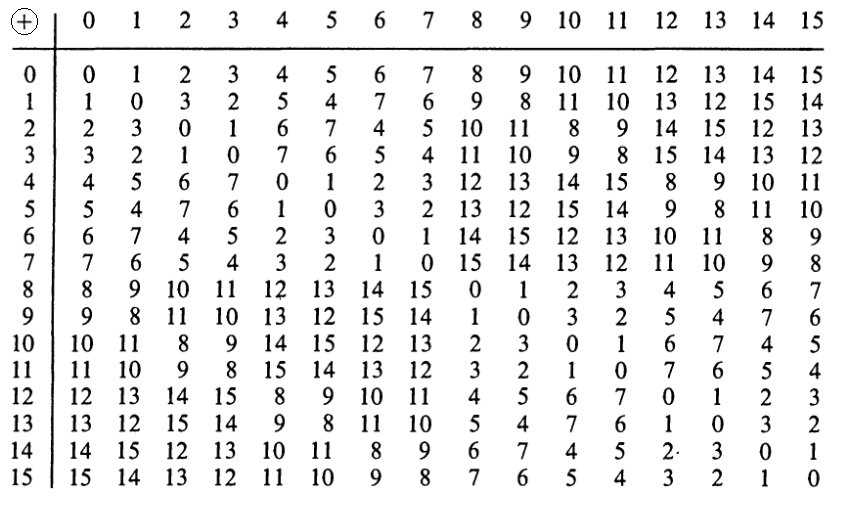
\includegraphics[scale=0.5,left]{nim_addition.png}
\end{figure}
\end{frame}

\begin{frame}{Producto}
	\begin{figure}
	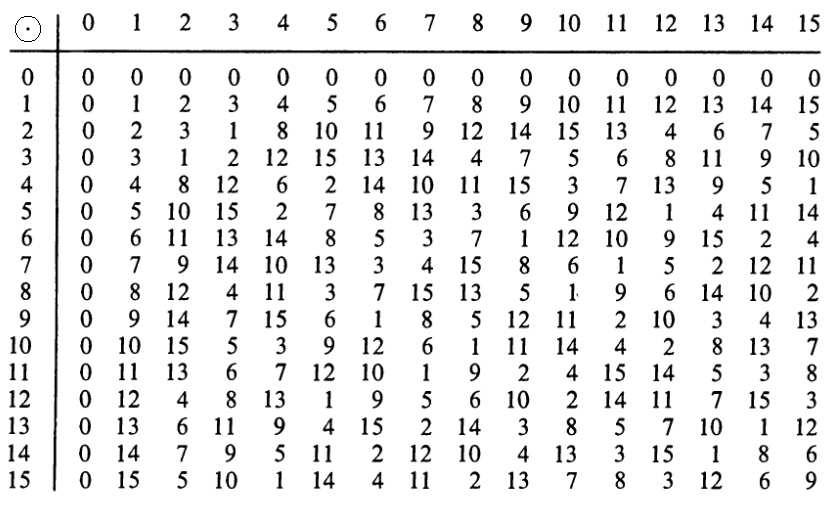
\includegraphics[scale=0.5,left]{nim_product.png}
	\end{figure}
\end{frame}

% Estas operaciones, cuando se ven en $\N$, son la suma y producto NIM de Teoría de Juegos y forman un cuerpo. Nosotros vamos a ver que se pueden extender a todos los ordinales.

% Antes de seguir quiero notar que estamos dándole una estructura de cuerpo a ON. En general se van a poder responder las preguntas que nos hagamos sobre un subcuerpo de ON (como sumar, multiplicar, dividir, buscar raíces de polinomios, o buscar elementos primitivos de alguna extensión de $F_2$ de manera efectiva, con algoritmos recursivos. Estos algoritmos recursivos, si responden la pregunta sobre cierto ordinal, van a reducir la pregunta a algo sobre un ordinal más chico. Como los ordinales forman un buen orden, al igual que $\N$, este algoritmo va a terminar!

% No tengo la menor idea si ON es "todas las extensiones de F_2 puestas todas juntas" jaja.

\begin{frame}{Formalización de la definición de las operaciones}

\begin{definition}[Suma]
	$\alpha \oplus \beta = min \{\gamma: \gamma \neq \alpha' \oplus \beta, \alpha \oplus \beta'\ \forall\ \alpha'<\alpha, \beta'<\beta \}$
	
	O, de manera más compacta:
	
	$\alpha \oplus \beta = mex\{ \alpha'\oplus\beta, \alpha\oplus\beta'\}$
\end{definition}
% Realmente la suma es el ordinal más chico posible que puede ser, porque si $\alpha+\beta = \alpha' + \beta$ entonces (si son un cuerpo) tachando los $\beta$ obtengo $\alpha = \alpha', absurdo.


\begin{definition}[Producto]

	$\alpha \odot \beta = mex\{ (\alpha'\odot \beta) \oplus (\alpha \odot \beta') \ominus (\alpha' \odot \beta')\}$
\end{definition}

% El producto se define así porque sino tenemos que $(\alpha - \alpha') (\beta - \beta') = 0$, o sea, no sería dominio integro.

\end{frame}


% Uno puede mirar segmentos de ordinales y preguntarse qué ordinales forman un grupo, un anillo, un cuerpo...

\begin{frame}{Simplest Extension Theorem}

(Notación: si $\gamma$ es un ordinal, escribimos $P_\gamma$ si lo queremos ver como conjunto)

Sea $\gamma$ un ordinal.

% Recordar que los ordinales son elementos y también conjuntos.
\begin{itemize}
	\item[$\bullet$]  Si $(P_\gamma, \oplus)$ no es un grupo, entonces $\gamma = \alpha \oplus \beta$, donde $(\alpha,\beta)$ es el par de ordinales más chico (en el orden lexicográfico) con $\alpha \oplus \beta \not\in P_\gamma$
	\item[$\bullet$]  Si $(P_\gamma, \oplus, \odot)$ es un grupo pero no es un anillo, entonces $\gamma = \alpha \odot \beta$, donde $(\alpha,\beta)$ es el par de ordinales más chico (en el orden lexicográfico) con $\alpha \odot \beta \not\in P_\gamma$
	\item[$\bullet$]  Si $(P_\gamma, \oplus, \odot)$ es un anillo pero no un cuerpo, entonces $\gamma \odot \alpha =1$, donde $\alpha$ es el ordinal más chico de $P_\gamma$ sin inverso en el conjunto.
	\item[$\bullet$]  Si $(P_\gamma, \oplus, \odot)$ es un cuerpo pero no es algebraicamente cerrado, entonces $\gamma$ es una raíz del polinomio más chico en el orden lexicográfico con ninguna raíz en $P_\gamma$
	\item[$\bullet$]  Si $(P_\gamma, \oplus, \odot)$ es un cuerpo algebraicamente cerrado, entonces $\gamma$ es el primer elemento trascendente sobre $P_\gamma$.
\end{itemize}

% ¡Choclo de texto! Esta slide no es para verla entera, pero todas las propiedades son parecidas y dicen que cada ordinal le va agregando estructura al conjunto considerado hasta ahora de la manera más simple posible.

% Y medio que pasa porque las operaciones dan como resultado el ordinal más simple posible

% Es más, también está pasando que los ordinales no son más que nombres que les ponemos a los elementos de $\overline{F_p}$. Si nos detenemos aquí no es muy sorprendente la cosa, pero el tema es que vamos a poder operar en este espacio. Esto nos lo dice el siguiente resultado:


%TODO en el communication se ve que la suma, el producto, y encontrar raíces de polinomios se puede hacer de manera efectiva.

\end{frame}


\begin{frame}{Simplest extension theorem, parte 2}

% Pasa algo muy lindo, que es que cuánta más estructura tengan los ordinales como conjuntos, más fácil es operar con ellos.

Sea $\gamma$ un ordinal.
\begin{itemize}
	\item[$\bullet$] Supongamos que $P_\gamma$ es un grupo. Entonces $\gamma \oplus \alpha = \gamma + \alpha\ \forall\ \alpha \in P_\gamma$ %Y realmente sabemos operar con las operaciones usuales (no requieren infinitos pasos)
	\item[$\bullet$]  Supongamos que $P_\gamma$ es un anillo y $\exists \delta \leq \gamma$ con $P_\delta$ un grupo tal que todo $\alpha \in \delta$ tiene inverso multiplicativo en $P_\gamma$ entonces: $\gamma \odot \alpha = \gamma \cdot \alpha \forall \alpha < \delta$
	\item[$\bullet$] Si $P_\gamma$ es un cuerpo y todo polinomio de grado $\leq n$ tiene raíz en $P_\gamma$ entonces $\displaystyle \bigoplus_{i=0}^n (\mathlarger{\gamma}^{\boxed{i}} \odot \alpha_i) = \sum_{i=0}^n \gamma^i \cdot \alpha_i$,
	$\forall \alpha_0,...,\alpha_n < \gamma$
\end{itemize}

% La intuición detrás de las demos es que cuánta más estructura tengan, 'mejor' puedo llenar los conjuntos sobre los que hago MEX y llenar todos los huecos.d

% Además, si estás cerca de un ordinal con estructura, es más fácil operar, porque el mex te hace necesitar operar con ordinales más chicos de manera recursiva. En algún sentido, tenés que bajar hasta el primer ordinal con suficiente estructura para no tener que hacer la cuenta

% Igual, en la vida real, hay algunos teoremas más que hacen que sumar y multiplicar sea realmente efectivo

% La suma es muuuy parecida a la suma NIM, y el producto es un asco y depende de unos $\alpha_p$ indexados por primos.


% La intuición detrás de las demos es que cuánta más estructura tengan, 'mejor' puedo llenar los conjuntos sobre los que hago MEX y llenar todos los huecos.d




\end{frame}


\begin{frame}{}

% $(ON,+,\cdot)$ es un cuerpo (con dominio una clase propia)

% Lo que Conway hace es quedarse con distintos segmentos de ON y se pregunta cuándo forman un grupo, un anillo, un cuerpo, un cuerpo algebraicamente cerrado, cuándo aparece el primer trascendente, etc.

% No nos vamos a meter en eso porque es un poco largo, pero quería mencionar cómo llega a construirse un cuerpo algebraicamente cerrado.

% Conway empieza con $\key{0,1}$ y considera extensiones cuadráticas, que corresponden a segmentos cada vez más grandes de ordinales. Itera el proceso hasta obtener un cuerpo cuadráticamente cerrado.

% Luego considera extensiones cúbicas de la clausura cuadrática, hasta conseguir una clausura cúbica, e itera con cada primo

% Conway tira un claim en el que dice que como el grupo de Galois de un cuerpo finito es abeliano, queda cuadráticamente cerrado después de considerar extensiones cúbicas, y así cuando pasás del enésimo primo al n+1-ésimo primo. Quiero explorar este claim.

% (También está la pregunta de por qué después de finalizar este proceso uno obtiene un cuerpo algebraicamente cerrado, pero como es una clausura de grado p-ésimo para cada primo, es más creíble esto)

\centering
\hspace*{-2.3cm}\vspace*{1cm}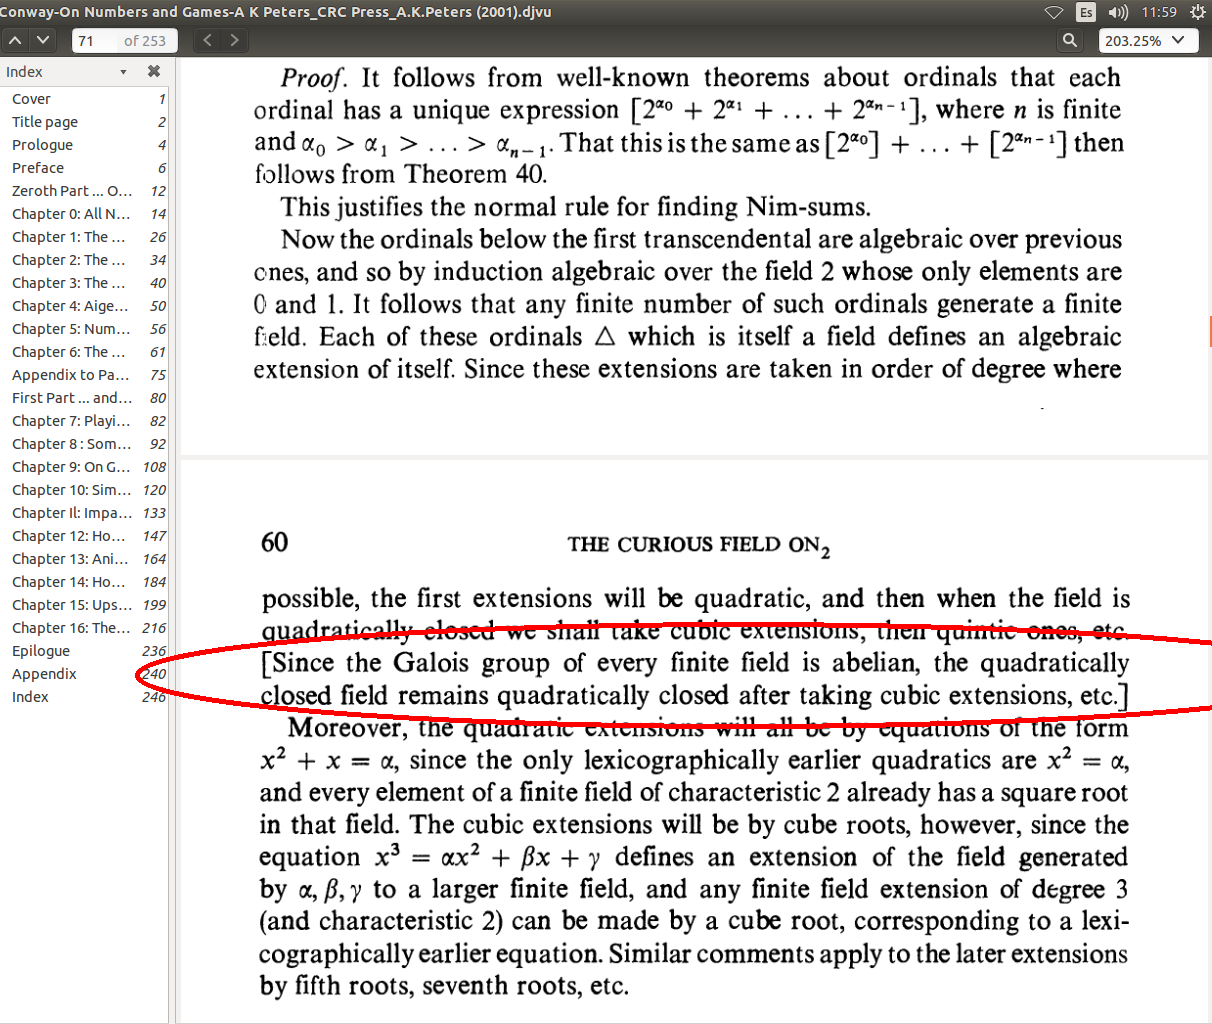
\includegraphics[scale=0.45]{claim.png}

\end{frame}



%TODO poner que 2^{2^n} coincide con F_{2^{2^n}}

\begin{frame}[fragile]{Demostración}

\small{Sea $E$ tal que no tiene polinomios irreducibles de grado $p$ y sea $L/E$ una extensión algebraica de $E$. Sea $f \in L[X]$ un polinomio de grado $p$ y supongamos que es irreducible. SPG, podemos suponer que $[L:K] < \infty$ porque de última lo cambiamos por K[coef/raíces de $f$] 
Sea $E=L(\alpha)$ con $\alpha$ una raíz de $f$. Luego $[E:L]=p$ y por lo tanto $p$ divide a $[E:K]$. Ahora bien, $E/K$ tiene Galois abeliano, y por el teorema de estructura para grupos abelianos, podemos obtener un subgrupo $H \subset(E/K)$ de índice $p$. Luego $E^H$ es una extensión de grado $p$. Pero esto era imposible, por como era $K$.}



\begin{center}
\begin{tikzcd}
E\arrow[dash]{d}{p} \arrow[dash]{dr}\\
L\arrow[dash]{d}{n} & E^H \arrow[dash]{dl}{p}\\
K\arrow[dash]{d}\\
\F_2\\
\end{tikzcd}
\end{center}
\end{frame}


\begin{frame}{Factorización de polinomios}

Analicemos el polinomio $x^3 - 2$. No se factoriza en $F_2$.

Afirmo que $\omega$ es raíz. En efecto, $\omega$ es la clausura cuadrática de $2$, así que es la solución del polinomio más simple que no tiene raíces en $\omega$. Ese polinomio es $x^3-2$, porque $x^3$ y $x^3-1$ se factorizan linealmente en $\omega$, y porque $2$ no tiene raíz cúbica en $\omega$. Veamos esta última afirmación:

$2 \odot 2 \odot 2 = 1$ así que si $\alpha$ es raíz cúbica de $2$ entonces tiene orden multiplicativo igual a $9$, y si $\alpha \in \omega \Rightarrow \alpha \in F_{2^{2^n}}$ para algún $n$. Pero el subgrupo multiplicativo de $F_{2^{2^n}}$ tiene índice $2^{2^n}-1$ y por inducción se ve que $0\not| 2^{2^n}-1 \forall n$. Luego $\alpha \not\in \omega$, entonces debe ser $\omega$.

Ahora, si uno hace Ruffini, obtiene $x^3-2 = (x-\omega) (x^2 + \omega x + \omega^2)$

\end{frame}

\begin{frame}
Analicemos $q(x) = x^2 + \omega x + \omega^2$.

Después de mucho pensar, intuí que una raíz debe 'estar cerca' de $\omega$ y propuse como solución $\omega \odot n$.

Enchufándolo en la ecuación y sacando factor común $\omega^2$ obtenemos que $q(x) = 0 \Leftrightarrow n^2 + n + 1 = 0$.

¡Y esta última ecuación es bien conocida! Es la que genera $F_{2^2} = 4$. Luego buscamos las raíces ahí y resulta que $2$ y $3$ son raíces.

Luego las raíces del polinomio original son $\omega, \omega \odot 2, \omega \odot 3$
\end{frame}



\begin{frame}{BIS, si me queda tiempo: dividir anda}

	Construimos los inversos inductivamente. Si ya existe $\frac{1}{\alpha'} \forall 0<\alpha'<\alpha$, entonces: \\
	
	Dado $\alpha, \beta = \frac{1}{\alpha} := mex\key{0,\frac{1+ (\alpha'-\alpha)\hat{beta}}{\alpha'} : \alpha' \neq 0}$ donde $\hat{beta}$ indica un elemento que ya ``metimos"\ en el conjunto. La idea es que tenés un ``sitio de construcción" donde podés usar los elementos anteriores para obtener nuevos elementos. Otra manera de definir al conjunto es diciendo que es el menor conjunto que contiene a $0$ y cerrado por $\frac{1+ (\alpha'-\alpha)\hat{\beta}}{\alpha'}$.
	
	Ahora bien, ¿qué pinta tienen estos elementos? Si $\hat{\beta}$ ya pertenece al conjunto, entonces un nuevo elemento $0\neq \doublehat{\beta}= \frac{1+ (\alpha'-\alpha)\hat{\beta}}{\alpha'} = \frac{1 + \alpha'\hat{\beta} - \alpha \hat{\beta}}{\alpha'}$
		
\end{frame}

\begin{frame}
	Multiplicando por $\alpha$ a ambos lados y luego componiendo con la función $1-x$ obtenemos $1 - \alpha \doublehat{\beta}= 1 - \alpha \frac{1 + \alpha'\hat{\beta} - \alpha \hat{\beta}}{\alpha'} = 1 - \frac{\alpha + \alpha \alpha'\hat{\beta} - \alpha^2 \hat{\beta}}{\alpha'} = \frac{\alpha' - \alpha - \alpha \alpha'\hat{\beta} + \alpha^2 \hat{\beta}}{\alpha'}$\\
	
	Analicemos la expresión $\alpha' - \alpha - \alpha \alpha'\hat{\beta} + \alpha^2 \hat{\beta}$. La podemos conmutar de modo que quede $\alpha' - \alpha\alpha'\hat{\beta} + \alpha^2\hat{\beta} - \alpha$, y sacando factor común obtenemos $\alpha'(1-\alpha\hat{\beta}) - \alpha(1 - \alpha\hat{\beta}) = (1-\alpha\hat{\beta}) ( \alpha'-\alpha)$. \\
	
	Juntando todo hemos obtenido $1-\alpha\doublehat{\beta}= (1-\alpha\hat{\beta}) \frac{\alpha'-\alpha}{\alpha'}$. Como el conjunto se construye inductivamente y $1-\alpha0 = 1 \neq 0$, tenemos que todo elemento $\hat{\beta}'$ cumple $1-\alpha\doublehat{\beta}\neq 0$.
\end{frame}


 \begin{frame}
 
	
	Ahora bien, aprovechando que $\doublehat{\beta}= \frac{1+ (\alpha'-\alpha)\hat{\beta}}{\alpha'}$, podemos hacer la siguiente cuenta: \\
	
	Un excluyente para $\alpha\beta$ va a ser de la forma $\alpha'\beta+\alpha\hat{\beta}-\alpha'\hat{\beta}$, y sabemos que $\doublehat{\beta}\alpha' = 1 + \alpha'\hat{\beta} - \alpha\hat{\beta} \Rightarrow \alpha\hat{\beta}-\alpha'\hat{\beta} = 1 - \hat{\beta}'\alpha'$.
	
	Luego tenemos que el excluyente va a ser de la forma $\alpha'\beta  + 1 - \hat{\beta}'\alpha' = \alpha'(\hat{\beta}-\hat{\beta}') + 1$.
	
	Esta cuenta nos dice que los excluyentes de $\alpha\beta$ son todos $\neq 1$, ya que $\beta, (\hat{\beta}-\hat{\beta}') \neq 0$.
	
	Además, si $\hat{\beta}= 0 \Rightarrow \doublehat{\beta}= \frac{1}{\alpha'}$ por la definición, así que el excluyente queda 0.
	
	Probamos que los ecluyentes de $\alpha\beta$ son todos distintos de $1$ y además está $0$, así que $\alpha\beta$ debe ser $1$.	

 \end{frame}


\begin{frame}{Bibliografía}

\begin{itemize}
	\item[$\bullet$] John H. Conway - On Numbers and Games (1976)
	\item[$\bullet$] Hendrik Lenstra - On the Algebraic Closure of Two (1977)
	\item[$\bullet$] [Graduate Studies in Mathematics] Aaron N. Siegel - Combinatorial Game Theory (2013, American Mathematical Society)
\end{itemize}
\end{frame}




\iffalse




% ---------------------------------------------------------------- %
% ---------------------------------------------------------------- %
% ---------------------------------------------------------------- %
% ---------------------------------------------------------------- %
% ---------------------------------------------------------------- %
% ---------------------------------------------------------------- %
% ---------------------------------------------------------------- %



%TODO importante:
% hablar de ordinales hasta w^w^w. La CNF nos da una notación para ellos
% Los ordinales representan buenos órdenes pero eso se medio abstracto
% teorema: todo buen orden se inyecta en un ordinal de von neumann
% pero como se construyen? de a uno, y tomando límite? inductivamente? es medio confuso.
% operaciones, exponenciación, cuidado con eso
% al final lo que pasa es que sabemos operar y comparar por la CNF de manera efectiva - existen programas que lo hacen, incluso! son algoritmos lineales en la cantidad de símbolos usadas para la notación.












% La idea de esta charla es contar un par de ideas usadas en la construcción hecha por Conway de la clausura algebraica de $F_2$ de manera efectiva, es decir, de modo que se pueda operar entre elementos del cuerpo.

% (Las ideas son cómo definir las operaciones naturales, y cómo ir cerrando el cuerpo)

% Para ello, vamos a usar ordinales.

% Los ordinales, a primera vista, no parecen llevarse muy bien con las palabras \textit{método efectivo}, al menos no es lo que yo pensé la primera vez que me los presentaron como "números transfinitos", diciéndome que eran muchos más que los cardinales y todo eso %TODO decir esto de manera menos bestia

%TODO agregar en otro lado (?): Además, Teresa, recuerdo que durante la cursada me preguntaste por qué eran útiles los ordinales. Esto que voy a contar intenta dar una posible respuesta.

%TODO agregar que conway escribió el libro en una semana

%TODO cuando hablo de MEX, escribirlo en columna (mínimo entero excluido) aparte, chiquito, en gris tal vez.

%TODO decir que la caracterización de $\bar{F_p}$ es canónica y natural. Pero por qué es canónica? Porque estoy usando ordinales, que "ya existen" en algún sentido? Porque sino uno va agregando $F_{p^n}$ y no sabe en qué orden? Revisar la página web de lo que saqué inicialmente la idea de la presentación, que hablaba de eso. Es por un tema de representanttes? ni idea

%TODO qué cuerpos algebraicamente cerrados conocemos, además de $\mathbb{C}$?

\begin{frame}{¿Qué son los ordinales?}

% Así como los cardinales identifican clases de equivalencia de conjuntos con la relación dada porque exista una biyección,
% Los ordinales identifican clases de equivalencia de conjuntos bien ordenados con la relación dada por biyecciones que respetan orden. (Morfismos de orden)

% La construcción de ordinales más clásica (y la que vamos a usar) es la dada por Von Neumann
\pause


%TODO escribir mejor formateado, por ejemplo con parentesis mas grande, en negrita los conjuntos y más débiles los que tienen al vacío
$$ 0 = \emptyset $$ \pause
$$ 1 = \key{0}$$ \pause
$$ 2 = \key{0,1}\ \ = 1 \cup \key{1} $$\pause
$$ 3 = \key{0,1,2} = 2 \cup \key{2}$$
$$ 4 = \key{0,1,2,3} = 3 \cup \key{3}$$

$$...$$

% Donde la manera de construirse un nuevo ordinal es considerar el conjunto de todos los ordinales anteriores. En ese sentido es una construcción inductiva.

\end{frame}

\begin{frame}{Más ordinales}
%TODO ¿esto está bien?
%TODO matchsticks representations, o postes de luz

$$5 = \key{0,1,2,3,4} = 4 \cup \key{4}$$
$$6 = \key{0,1,2,3,4,5} = 5 \cup \key{5}$$ \pause
$$\omega = \key{0,1,2,3,...}$$ \pause
$$\omega + 1 = \key{0,1,...,\omega} = \omega \cup \key{\omega}$$
$$\omega + 2 = \key{0,1,...,\omega, \omega+1} = \omega \cup \key{\omega+1}$$
$$...$$ \pause
$$\omega \cdot 2 = \key{0,1,...,\omega, \omega+1, \omega+2,...}$$
\end{frame}


\begin{frame}{Una representación gráfica hasta $\omega^\omega$}
	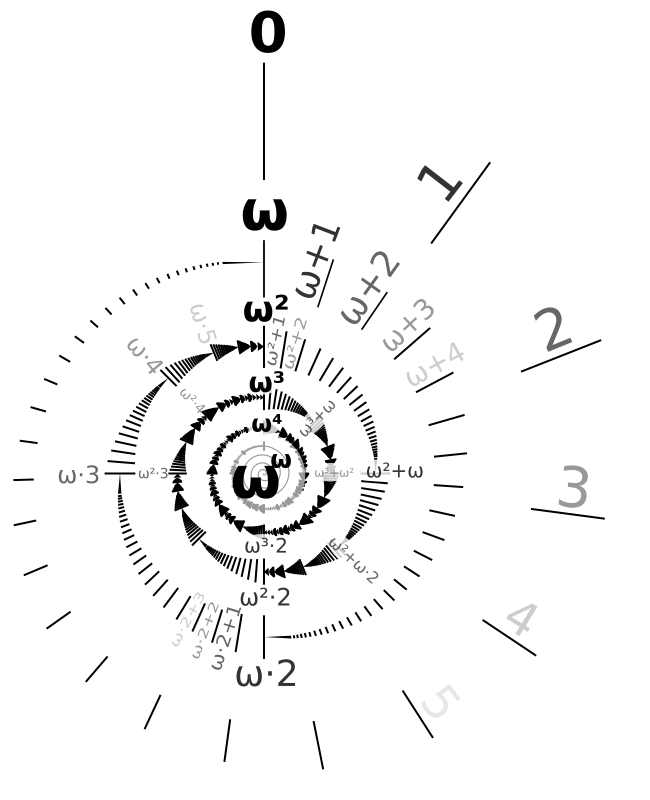
\includegraphics[scale=0.42]{spiral.png}
\end{frame}

% Los ordinales se dividen en dos grandes grupos: ordinales que son el siguiente de otro ordinal (es decir, que tienen un inmediato anterior), y ordinales que no, como $\omega$, ó $\omega + \omega$, que es el límite de hacer $\omega + n$. A estos últimos se los llama ordinales límite (y se los puede ver, en efecto, como un límite)

\begin{frame}{Inducción transfinita}

% Como todo ordinal es un siguiente, o es la unión de los anteriores a él, surge un esquema de demostración llamado inducción transfinita

%TODO Escribirlo mejor!

\begin{itemize}
	\item[$\bullet$]Si vale $P(0)$
	\item[$\bullet$]Si vale $P(\alpha) \Rightarrow P(\alpha + 1)$
	\item[$\bullet$]Si $\alpha$ es un ordinal límite y $P(\lambda)\ \forall\ \lambda < \alpha \Rightarrow P(\cup_{\lambda<\alpha} \lambda)$
\end{itemize}

entonces P vale para todo ON.

% Porque supongamos que no vale para todo ON. Entonces hay un ordinal mínimo para el cuál no vale...

\end{frame}


\begin{frame}{Operaciones con ordinales}

% Existen ciertas operaciones clásicas con ordinales,
% la suma, el producto, y la exponenciación, que nos permiten obtener ordinales más grandes

% Estas operaciones son una extensión de las usuales de números naturales, y en ese sentido los ordinales se pueden pensar como números nuevos, que extienden la aritmética usual de \N

Si $\alpha,\beta$ son ordinales:

La suma entre $\alpha$ y $\beta$ se define como el (buen) orden correspondiente a $\alpha \cup \beta$.

El producto entre $\alpha$ y $\beta$ se define como el (buen) orden lexicográfico correspondiente al producto cartesiano entre los conjuntos. \pause

Ambos son análogos a la suma y producto de cardinales.

\end{frame}

\begin{frame}{Exponenciación}
	%La exponenciación también se define inductivamente (si para definir $\alpha^\beta$ intentáramos dar un buen orden a las funciones $f : \beta \rightarrow \alpha$ fallaríamos)
	\pause	
\begin{itemize}
	\item[$\bullet$]$\alpha^0:= 1$
	\item[$\bullet$]$\alpha^{\beta + 1} := \alpha^\beta \cdot \alpha$
	
	%TODO explayarse https://en.wikipedia.org/wiki/Ordinal_arithmetic#Exponentiation
	\item[$\bullet$]Si $\beta$ es límite, $\alpha^\beta = \underset{\lambda < \beta}{\cup} \alpha^\lambda$.
\end{itemize}


\end{frame}


\begin{frame}{Forma normal de Cantor}

Todo ordinal $0 \neq \beta$ que nos va a interesar (o sea, no muy grande) admite una expresión de la siguiente forma:


%PIZARRÓN: aclarar que "no muy grande" es que esté debajo de $\varepsilon_0$

$$\beta = \omega^{\alpha_1} \cdot m_1 + ... + \omega^{\alpha_k} \cdot m_k$$

con $\beta > \alpha_1 > ... > \alpha_k$, y $\m_i \in \N$

Esto es una descomposición de $\beta$ en ordinales más chicos que él. \bigskip \pause

% Además, los $\alpha_i$ también se van a poder descomponer en ordinales más chicos. Esta cadena de descomposiciones me da una secuencia de ordinales decrecientes $\beta_1 > \beta_2 > ....$ Ahora, al principio vimos que cada ordinal es el conjunto de ordinales más chicos que él. $\forall\i > 1, \beta_i \in \beta_1$, que es un buen orden. Entonces eventualemente la secuencia termina, no puede descender infinitamente. Esto quiere decir que esta descomposición que hacemos termina.

% Notar el parecido con $\N$, que también está bien ordenado y por eso podemos factorizar en primos.

% Lo que obtenemos es ordinales escritos como arbolitos, usando el símbolo $\omega$, y números naturales.

Algunos ejemplos:

$\omega\textbf{,}\ \ \omega^\omega \cdot 2\textbf{,}\ \ \omega^{\omega^2} + \omega^\omega + 4\textbf{,}\ \ \omega^{\omega^{\omega^2} + 2}$

% Lo importante de todo esto es que podemos operar y comparar ordinales de manera efectiva porque tenemos una notación para ellos. (No vamos a ver cómo se opera pero es muy fácil)

% Sobre eso es mi tesis. Como cada ordinal se identifica con el conjunto de todos los ordinales anteriores, el primer ordinal no numerable (por ser el primero) es el conjunto de todos los ordinales numerables. Luego hay no numerables ordinales numerables.

% Eso hace que sea literalmente imposible nombrarlos a todos, pero hay distintas notaciones para segmentos de los ordinales. La de recién era una. Por notación me refiero a maneras de nombrar ordinales hasta cierta altura, digamos, con finitos símbolos, de manera única, y de modo que sea fácil comparar y operar ordinales escritos en esa notación

% Lo que vamos a asumir en esta charla es que "se puede" con los que vamos a usar.


\end{frame}

\begin{frame}{Algunos problemas de las operaciones clásicas}


\begin{itemize}
	\item[$\bullet$]En general no son conmutativas: $1 + \omega \neq \omega + 1$
	\item[$\bullet$]????? %TODO algo más?
\end{itemize}

\end{frame}

\begin{frame}{Las operaciones naturales de Conway}

%TODO decir que Conway escribió su libro en una semana

% Conway definió otra suma y otro producto, las llamadas "operaciones naturales" de ordinales.

% Él buscaba las operaciones más simples que hicieran de On un cuerpo.

% Restrinjámonos primero a los números naturales.
% Supongamos que estamos armando la tabla de doble entrada de la suma de ordinales.
% Y que supongamos que ya están definidos $\alpha'+\beta, \alpha + \beta'$ (explicar los primas) entonces $\alpha+\beta$ es el ordinal más chico consistente con la tabla de suma de algún cuerpo (que contenga a los elementos). Lo mismo va a pasar con la tabla de multiplicación.

%PIZARRÓN: hacer ejemplo en el pizarrón. Como 1+1=0, ya queda de entrada que el cuerpo va a ser de característica 2.

%TODO son los ordinales debajo de $\omega$ un cuerpo? Creo que sí, y es cuadráticamente cerrado. Lo dice Conway

%TODO acá no hay nada, completar el frame con algo útil.

\end{frame}

\begin{frame}
\begin{figure}
	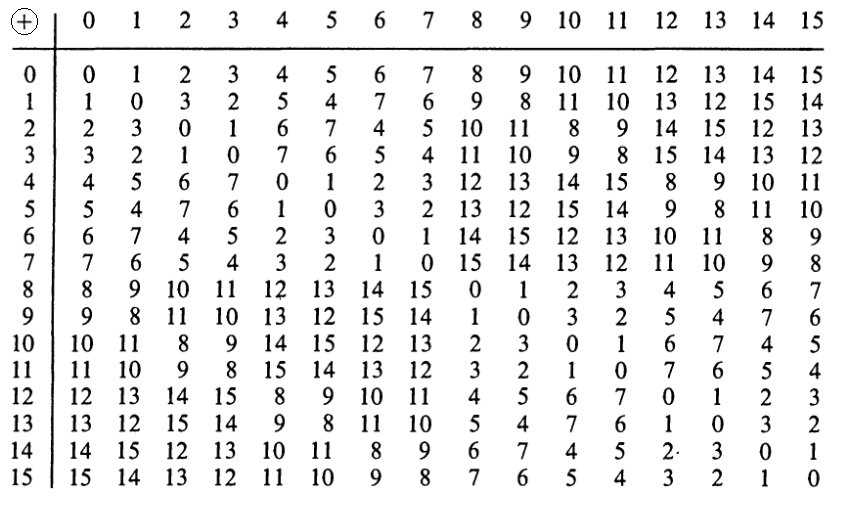
\includegraphics[scale=0.5,left]{nim_addition.png}
\end{figure}
\end{frame}

\begin{frame}{Producto}
	\begin{figure}
	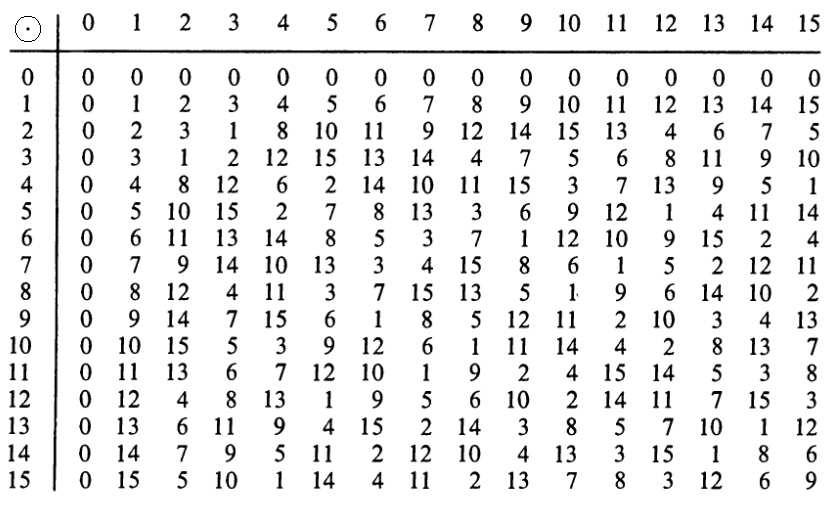
\includegraphics[scale=0.5,left]{nim_product.png}
	\end{figure}
\end{frame}

% Estas operaciones, cuando se ven en $\N$, son la suma y producto NIM de Teoría de Juegos y forman un cuerpo. Nosotros vamos a ver que se pueden extender a todos los ordinales.

% Antes de seguir quiero notar que estamos dándole una estructura de cuerpo a ON. En general se van a poder responder las preguntas que nos hagamos sobre un subcuerpo de ON (como sumar, multiplicar, dividir, buscar raíces de polinomios, o buscar elementos primitivos de alguna extensión de $F_2$ de manera efectiva, con algoritmos recursivos. Estos algoritmos recursivos, si responden la pregunta sobre cierto ordinal, van a reducir la pregunta a algo sobre un ordinal más chico. Como los ordinales forman un buen orden, al igual que $\N$, este algoritmo va a terminar!

% No tengo la menor idea si ON es "todas las extensiones de F_2 puestas todas juntas" jaja.


\begin{frame}{Formalización de la definición de las operaciones}

%TODO pasarlo a español
\begin{definition}[Suma]
	$\alpha + \beta = min \{\gamma: \gamma \neq \alpha' + \beta, \alpha + \beta'\ \forall\ \alpha'<\alpha, \beta'<\beta \}$
	
	O, de manera más compacta:
	$\alpha + \beta = mex\{ \alpha'+\beta, \alpha+\beta'\}$
\end{definition}

% Realmente la suma es el ordinal más chico posible que puede ser, porque si $\alpha+\beta = \alpha' + \beta$ entonces (si son un cuerpo) tachando los $\beta$ obtengo $\alpha = \alpha', absurdo.

\begin{theorem}[Los ordinales forman un grupo abeliano]
	\begin{itemize}
		\item[]
		\item[$\bullet$]$\alpha + \beta = \beta + \alpha$
		\item[$\bullet$]$\alpha + \beta = \alpha + \gamma \Leftrightarrow \beta = \gamma$
		\item[$\bullet$]$\alpha + \beta = 0 \Leftrightarrow \alpha = \beta$
		\item[$\bullet$]$\alpha + 0 = \alpha$
		\item[$\bullet$]$(\alpha + \beta) + \gamma = \alpha + (\beta + \gamma)$
		\item[$\bullet$]$\alpha + \alpha = 0, -\alpha = \alpha$
	\end{itemize}
\end{theorem}

%TODO la demo puede ser en el pizarrón.
% Voy a hacer dos demos, con suerte

\end{frame}


\begin{frame}

%TODO contar sobre $F_2^{2^k},F_2^{3^k}$,...y que así se va construyendo.

%TODO elementos primitivos?

%TODO en el communication se ve que la suma, el producto, y encontrar raíces de polinomios se puede hacer de manera efectiva.

Se va clausurando de a poco, pero por teorema que voy a hacer en el pizarrón, una extensión de una clausura p-ésima sigue quedando p-ésimamente clausurada.

...y todo es Galois, así que eso prueba que después de hacerlo para todo primo queda algebraicamente cerrado...

Esto creo que se ve por el absurdo.

Supongamos que no es algebraicamente cerrado, entonces considero una extensión de grado $n$, como es Galois (revisar si esto vale) puedo considerar una subextensión (estricta) de grado $p$ con $p|n$, pero entonces no me salí del cuerpo, absurdo.

Revisar, porque creo que estoy usando que es Galois, lo cuál es bastante copado. Valía que toda extensión (algebraica?) de cuerpos finitos es Galois? O solo si el grado es finito? Creo que $Gal(\bar{F_p}/F_p)$ es cíclico (generado por el automorfismo de Frobenius? Revisar) Esto debe estar mal... Pero si es cíclico es abeliano entonces todo subgrupo es normal y me define (si todo es lindo y separable) una subextensión Galois.

....pero hay algo que no me cierra!! Porque si el grado de la extensión es infinita no puedo concluir nada, creo.


\end{frame}


\begin{frame}{}

% $(ON,+,\cdot)$ es un cuerpo (con dominio una clase propia)

% Lo que Conway hace es quedarse con distintos segmentos de ON y se pregunta cuándo forman un grupo, un anillo, un cuerpo, un cuerpo algebraicamente cerrado, cuándo aparece el primer trascendente, etc.

% No nos vamos a meter en eso porque es un poco largo, pero quería mencionar cómo llega a construirse un cuerpo algebraicamente cerrado.

% Conway empieza con $\key{0,1}$ y considera extensiones cuadráticas, que corresponden a segmentos cada vez más grandes de ordinales. Itera el proceso hasta obtener un cuerpo cuadráticamente cerrado.

% Luego considera extensiones cúbicas de la clausura cuadrática, hasta conseguir un cuerpo cúbicamente cerrado, e itera con cada primo

% Conway tira un claim en el que dice que como el grupo de Galois de un cuerpo finito es abeliano, queda cuadráticamente cerrado después de considerar extensiones cúbicas, y así cuando pasás del enésimo primo al n+1-ésimo primo. Quiero explorar este claim.

% (También está la pregunta de por qué después de finalizar este proceso uno obtiene un cuerpo algebraicamente cerrado, pero como es una clausura de grado p-ésimo para cada primo, es más creíble esto)

\centering
\hspace*{-2.3cm}\vspace*{1cm}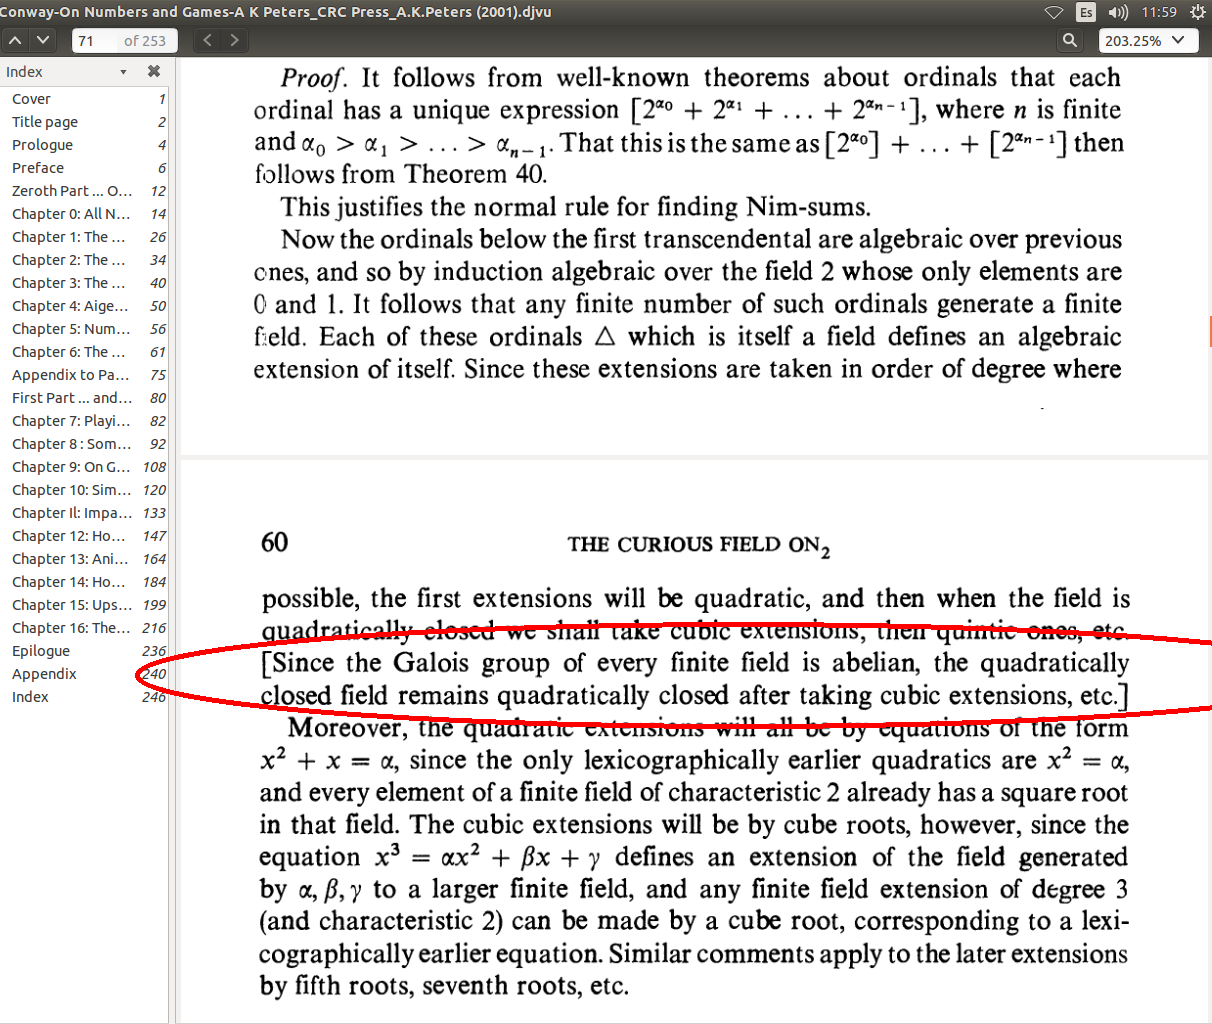
\includegraphics[scale=0.45]{claim.png}

\end{frame}

\begin{frame}
(demostración que pensé con juampi y saqué de mse)
\end{frame}

\begin{frame}{BIS, si me queda tiempo: dividir anda}

La demo es genial, no sé si hacerla o seguir con cuerpos. Le voy a preguntar a Teresa si se la puedo entregar en una hoja aparte.

\end{frame}












% ---------- BORRADOR DE CHARLA -----------------%


\begin{frame}{¿Qué son los ordinales?}
	Definición de ordinales sucesores y ordinales límite.
	
	Resaltar que cada ordinal se identifica con el conjunto de ordinales menores que él. Empezar con los finitos, pasar a $\omega, 2\cdot \omega$
\end{frame}

\begin{frame}{Inducción transfinita}
	¿En qué contexto estamos? ¿Vale hacer inducción transfinita? ¿Qué significa que valga? ¿La inducción es un axioma?
\end{frame}

\begin{frame}{Operaciones básicas: suma y producto}

\end{frame}

\begin{frame}{Exponenciación}


% ¿Por qué te queda numerable?
\end{frame}

% Esto probablemente se vaya
\begin{frame}{$\omega^\omega$}
	Unión numerable; libros.
\end{frame}

% Esto probablemente se vaya
\begin{frame}{$\omega^{\omega^\omega}$}
	Forma normal de Cantor, polinomios. Uff
\end{frame}

\begin{frame}{Las operaciones naturales de Conway}
	Conway quería que fueran un cuerpo. Definición de suma y producto naturales. Por qué son así. Algunos ejemplos
\end{frame}

\begin{frame}{Suma}	
	\begin{figure}
	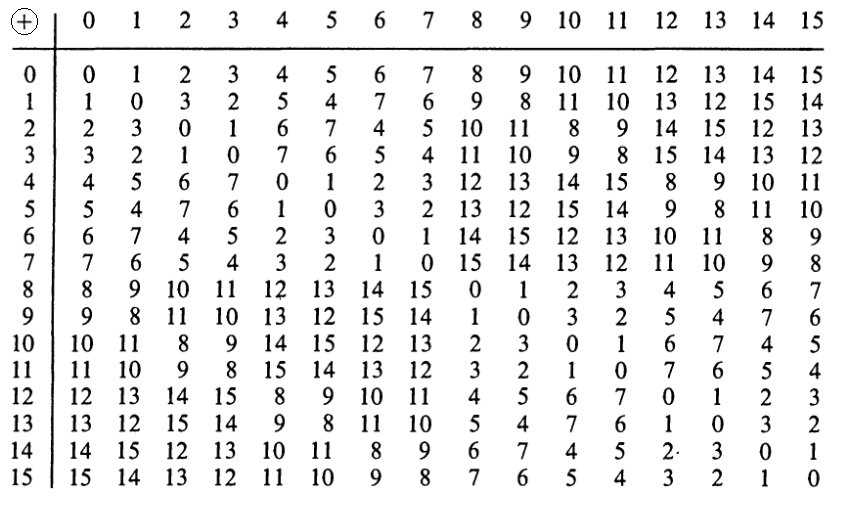
\includegraphics[scale=0.5,left]{nim_addition.png}
	\end{figure}
\end{frame}

\begin{frame}{Producto}
	\begin{figure}
	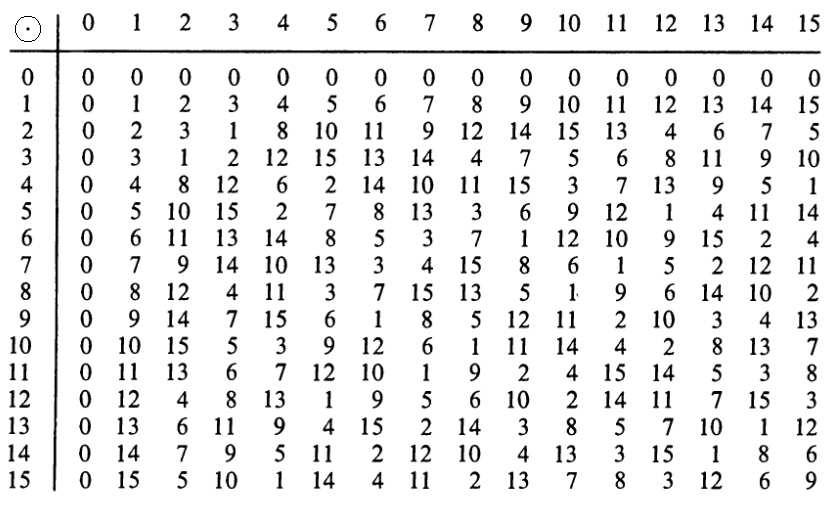
\includegraphics[scale=0.5,left]{nim_product.png}
	\end{figure}
\end{frame}

\begin{frame}{$(ON,+,\cdot)$ es un cuerpo (con dominio una clase propia)}
	Probemos algunas de las propiedades que deberíamos ver:
	
	% Por qué no puedo ver los puntos? Este theme es una garcha
	\begin{itemize}
		\item[$\bullet$]La suma es conmutativa
		\item[$\bullet$]El producto es asociativo: por inducción transfinita en $\underset{\sigma \in S_3}{max}[\sigma(\alpha) + \sigma(\beta) + \sigma(\gamma)]$
		\item[$\bullet$]Todo elemento tiene inverso
	\end{itemize}
\end{frame}

\begin{frame}{Todo elemento tiene raíz cuadrada}
	$\beta = \sqrt{\alpha} = mex \{\sqrt{\alpha'}, \frac{\beta'\beta^* + \alpha}{\beta'+\beta^*}\}$, donde $\beta'\neq \beta^*$ son dos elementos que ya estaban en el conjunto en una iteración previa.
\end{frame}

%Esto va sin demostración
\begin{frame}{Las operaciones usuales y las naturales se llevan bien}


\begin{theorem}
	Si $\Delta$ es un grupo entonces $[\Delta\alpha] + \beta = [\Delta\alpha+\beta]\ \forall \alpha,\beta\in\Delta$
\end{theorem}

% Este tal vez está bueno probarlo
\begin{theorem}
	Si $\Delta$ es un anillo y $\Gamma \leq \Delta$ es un subgrupo aditivo tal que $\forall \gamma\in \Gamma, \gamma\m \in \Delta$ entonces $\Delta\gamma = [\Delta\gamma] \forall\gamma\in\Gamma$
\end{theorem}
\end{frame}

% Cada ordinal extiende al objeto anterior de la manera más simple posible

\begin{frame}
	\begin{theorem}
		Si $\Delta$ es un cuerpo que no es algebraicamente cerrado entonces $\Delta$ es raíz del primer polinomio (en el orden lexicográfico) que no tiene raíz en $\Delta$
	\end{theorem}
\end{frame}

\begin{frame}{no creo que no haga ninguna cuenta sobre la clausura algebraica}
\end{frame}

%TODO preguntar por qué si un cuerpo es cuadráticamente cerrado y su grupo de Galois es abeliano entonces una extensión cúbica también es cuadráticamente cerrado


\begin{frame}
Creo que no voy a hacer la demo del teorema propiamente dicha pero voy a contar que necesito usar lo siguiente e intentar demostrarlo:

[Since the Galois group of every finite field is abelian, the quadratically
closed field remains quadratically closed after taking cubic extensions, etc.]	


\end{frame}

\begin{frame}

Igual la verdad no entiendo por qué al agregar de a una las raíces obtengo todo. Tiene que ver con extensiones resolubles, o algo así....pero en el caso muy particular de cuerpos finitos.

A ver, un intento: si agrego de a uno los elementos sin raíz cuadrada, cuando considero la extensión generada por todos esos elementos cada elemento que agregué tiene raíz cuadrada.

NO. Ya entendí; en cada paso le estoy agregando al cuerpo las raíces de los polinomios de grado 2. Que en realidad hay uno solo, que es $x^2+x$ porque aparentemente todo elemento tiene raíz cuadrada.

Creo.

¿Valdrá por la unicidad de las extensiones de $F_2$? Me parece que sí. Porque valía $F_{q^n} \subset F_{q^m} \Leftrightarrow n|m$, y para ver que lo que obtengo es, por ejemplo, cuadráticamente cerrado, le puedo agregar a $F_{q^n}$ la raíz de un polinomio de grado 2 y necesariamente la extensión va a coincidir con $F_{q^{2n}}$, que es agregar al siguiente tipito.

La cuenta de por qué esto vale la debería tener bien escrita por si Teresa me pregunta.

\end{frame}


\begin{frame}{Cuento que se puede operar}
	Los polinomios en $\omega^{\omega^\omega}$ se evalúan normalmente! Pará, esto es re mentira, porque diría que las operaciones coinciden :/
	Creo que lo que pasa es que podés evaluar en ordinales que son un cuerpo.
\end{frame}

\begin{frame}
	Me parece que lo mejor va a ser enunciar el teorema  49 y calcular algún $\alpha_p$
\end{frame}

\fi
\end{document}

%
%\tableofcontents
%\part{Addition and Subtraction}
%\chapter{Addition} \chaptercontent
%\chapter{Subtraction} \chaptercontent
%\part{Multiplication and Division}
%\chapter{Multiplication} \chaptercontent
%\chapter{Division} \chaptercontent
